\subsection{Installation, Running and Original Copy Protection} \label{subsection:android-copy}
%START TEXT INPUT
This is my real text! Rest might be copied or not be checked!
%START TEXT INPUT

%
Installation two steps:  primary is the APK verification and secondary is the bytecode optimization\newline
legitimate signature as well as correct classes.dex structure cannot be verified are rejected for installation by the OS\newline
Once verified, the .dex file is forwarded for optimization: a necessary step due to the high diversity of Android running hardware (dex)-see- Dalvik executable is a generic file format which needs additional processing to achieve best performance for the concrete device architecture (odex)\newline
optimization\newline
step removes the classes.dex from the original APK archive and loads in memory the .odex file upon execution, occurs only once, during the initial run of the application which explains the usually slower first application launch comparing to the subsequent ones

ablauf starten von app\newline
When an Android application is executed, the process consists of the following four parts:
• Dalvik bytecode, which is located in the dex file
• Dalvik Virtual Machine [13], which executes the Dalvik bytecode
• Native Code, like shared objects, which is executed by the processor
• Android Application Framework, which provides services for the application\newline
\cite{kovachevaMaster}
%
\begin{figure}[h]
    \centering
    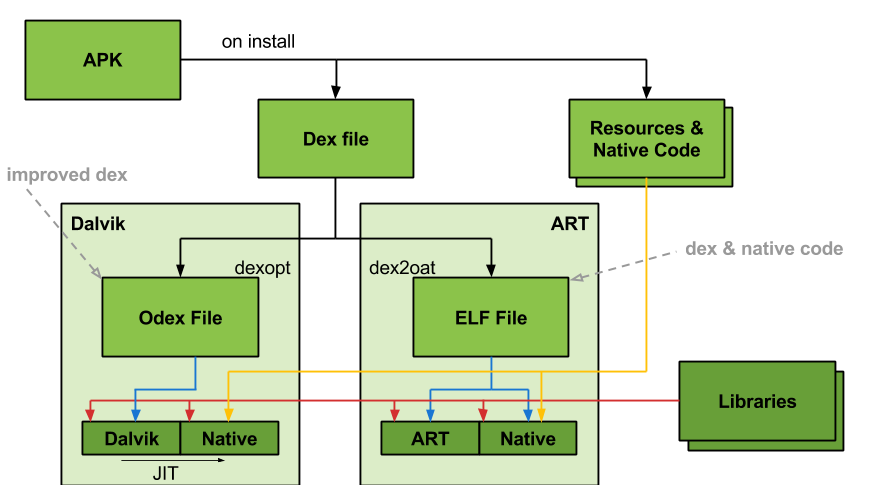
\includegraphics[width=0.8\textwidth]{data/install.png}
    \caption{install}
    \label{fig:install}
\end{figure}

%
unauthorized usage of an app through copy protection
apk was installed in a location on the phone /data/app user could not access
useless if single user can get apk and redistribute, gained by root
successful as long as root was not easy for everyone -see- samsung rooting odin QUELLE, did not have too big impact as today, oneclick root kits QUELLE, standard for nexus

on install app's classes.dex is copies an optimized version (odex) to dalvik cache /data/dalvik-cache/, for faster startup (contains system apps and frameworks as well)
odex erklären, byteswapping, structure realigning and memory-mapping
when app is started optimized code from dalvik cache will be executed instead of apk
\cite{munteanLicense}
%

%
The Android operating system is a multi-user Linux system in which each app is a different user.
By default, the system assigns each app a unique Linux user ID (the ID is used only by the system and is unknown to the app). The system sets permissions for all the files in an app so that only the user ID assigned to that app can access them
Each process has its own virtual machine (VM), so an app's code runs in isolation from other apps.
By default, every app runs in its own Linux process. Android starts the process when any of the app's components need to be executed, then shuts down the process when it's no longer needed or when the system must recover memory for other apps

\cite{developerFundamentals}
%

old system was to put APK in folder user cannot access, unless you root
weak, almost non-existant, anyone who can copy it can distribute it


It replaces the old system copy protection system, wherein your APKs would be put in a folder that you can't access. Unless you root. Oh, and anyone who can copy that APK off can then give it to someone else to put on their device, too. It was so weak, it was almost non-existant.\newline
kann mit root umgangen werden


Im original vom Markt direkt rutnergeladen und dann wird sie an den ort geschoben und kann nicht mehr zugegriffen werden -see- rechte etc, QUELLE\newline
